\documentclass[tikz,border=6pt]{standalone}
\usepackage{tikz}

\begin{document}

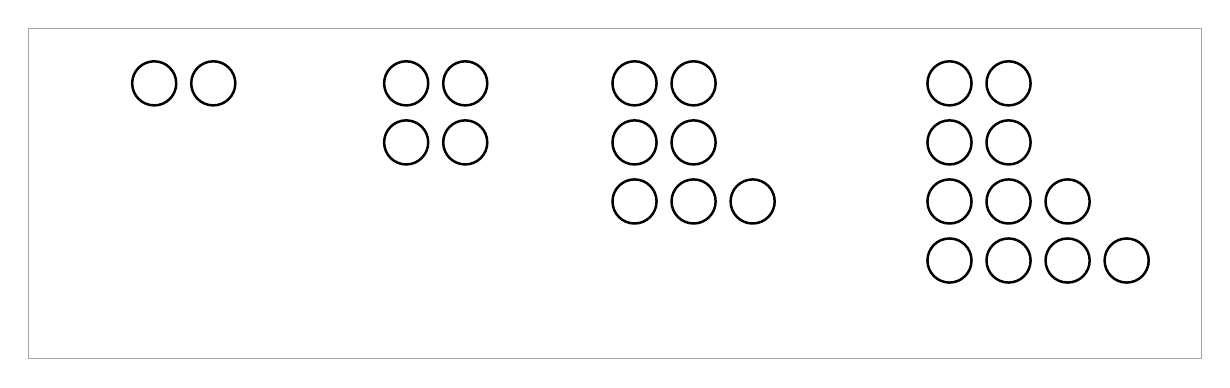
\begin{tikzpicture}[line cap=round,line join=round]
  % --- parameters ---
  \def\s{0.75}      % grid step (cm-ish)
  \def\r{0.28}      % circle radius

  % --- outer frame ---
  \draw[gray!70] (-0.7,0.9) rectangle (14.2,-3.3);

  % Common style
  \tikzset{dot/.style={draw=black,line width=.9pt}}

  % ========== (1) : 2 circles ==========
  \begin{scope}[shift={(0.9,0.2)}]
    \foreach \x/\y in {0/0,1/0}
      \draw[dot] (\x*\s,\y*\s) circle (\r);
  \end{scope}

  % ========== (2) : 4 circles ==========
  \begin{scope}[shift={(4.1,0.2)}]
    \foreach \x/\y in {0/0,1/0,0/-1,1/-1}
      \draw[dot] (\x*\s,\y*\s) circle (\r);
  \end{scope}

  % ========== (3) : 7 circles (2,2,3) ==========
  \begin{scope}[shift={(7.0,0.2)}]
    \foreach \x/\y in {0/0,1/0,0/-1,1/-1,0/-2,1/-2,2/-2}
      \draw[dot] (\x*\s,\y*\s) circle (\r);
  \end{scope}

  % ========== (4) : 11 circles (2,2,3,4) ==========
  \begin{scope}[shift={(11.0,0.2)}]
    \foreach \x/\y in {0/0,1/0,0/-1,1/-1,0/-2,1/-2,2/-2,0/-3,1/-3,2/-3,3/-3}
      \draw[dot] (\x*\s,\y*\s) circle (\r);
  \end{scope}
\end{tikzpicture}

\end{document}
